%%%%%%%%%%%%%%%%%%%%%%%%%%%%%%%%%%%%%%%%%%%%%%%%%%%%%%%%%%%%%%%%%%%%%%%%%
%
% File: candidacy_paper.tex
%
% Author: A. J. Tropiano (tropiano.4@osu.edu)
% Date: July 1, 2019
%
% Candidacy paper on the status of nuclear optical potentials and future prospects.
%
% Revision history:
% 	07/02/19 --- Starting with bulleted outline.
%     07/10/19 --- Adding equations to formalism section.
%	07/11/19 --- Put theoretical issues section as part of the conclusion. Also, wrote much of the formalism section.
%	07/15/19 --- Wrote the phenomenology section.
%	07/17/19 --- Wrote the introduction section.
%	07/19/19 --- Wrote microscopic optical potentials section.
%	07/25/19 --- Revised draft from introduction through multiple-scattering approach.
%	07/26/19 --- Revised nucleon self-energy section and wrote conclusion.
%     07/29/19 --- Finalized paper.
%	08/01/19 --- Correct minus sign typo in first optical potential equation.
%
%%%%%%%%%%%%%%%%%%%%%%%%%%%%%%%%%%%%%%%%%%%%%%%%%%%%%%%%%%%%%%%%%%%%%%%%%


\documentclass[preprintnumbers,floatfix,aps,prc,preprint,nofootinbib]{revtex4-1}

% Packages
\usepackage{amsmath}
\usepackage{amsfonts}
\usepackage{amssymb}
\usepackage{bm}
\usepackage[font=small,skip=0pt]{caption} % For captions on figures and tables
\usepackage{cellspace}
\usepackage{color}
\usepackage{enumerate}
\usepackage{epsfig}
\usepackage[figuresright]{rotating}
\usepackage{float}
\usepackage{hyperref} % For clickable links to sections within table of contents
\usepackage{graphicx}
\graphicspath{{../../../Figures/Pictures/}} % Setting the graphics path
\usepackage{physics} % For bra-ket notation
\usepackage{siunitx}
\usepackage[caption=false]{subfig} % For sub-figures

\newcommand{\eps}{\varepsilon}


\begin{document}


%%%%%%%%%%%%%%%%%%%%%%%%%%%%%%%%%%%%%%%%%%%%%%%%%%%%%%%%%%%%%%%%%%%%%%%%%
\title{Status of nuclear optical potentials and future prospects}


\author{A.~J.~Tropiano}

\affiliation{\mbox{Department of Physics, The Ohio State University, Columbus, OH 43210, USA}}

\date{\today}

\begin{abstract}
We review current progress on nuclear optical potentials emphasizing the successes and limitations of several approaches. We present the basic formalism of the nuclear optical model as derived by Feshbach \cite{Feshbach:1958nx, Feshbach:1962ut}. We give an overview of phenomenological models and two microscopic approaches involving multiple-scattering and nucleon self-energy. We discuss key theoretical issues for these approaches and future work.
\end{abstract}

\maketitle

\newpage


%%%%%%%%%%%%%%%%%%%%%%%%%%%%%%%%%%%%%%%%%%%%%%%%%%%%%%%%%%%%%%%%%%%%%%%%%
\section{Introduction}
\label{sec:intro}


Nuclear reactions are central to many areas of physics. A good understanding of these processes is necessary to answer questions such as the origin of the heavy elements in the universe, fundamental symmetries, or the limits of nuclear stability. For example, half of the neutron-rich atomic nuclei past iron on the periodic table are created by the rapid neutron-capture process known as the r-process which involves a series of nuclear reactions even with nuclei that have never been experimentally produced. Construction of an ``r-process laboratory'' is underway, the Facility for Rare Isotope Beams (FRIB), which seeks to produce many exotic, neutron-rich isotopes (isotopes are nuclei with fixed proton number and varying neutron number) and measure new data to better understand the areas mentioned above. Fig.~\ref{fig:nuclear_chart_2018} shows nuclei with the neutron number, N, on the x-axis and the proton number, Z, on the y-axis with stable nuclei as black squares. The r-process takes place below the line of stability with exotic, neutron-rich nuclei, which is the region where FRIB is expected to make substantial progress. It is critical to understand nuclear reactions since facilities must use reactions to produce and study short-lived exotic nuclei.
\\

From the theoretical side, the task is to solve the nuclear scattering problem, that is, a projectile particle scattering from a target nucleus interacting via the strong force. Typically, projectile particles consist of protons, neutrons, $\alpha$ particles, or nuclei. Scattering from a nuclear target leads to a quantum many-body problem since nuclei are composite particles composed of protons and neutrons meaning the projectile interacts with several nucleons in the target nucleus. This presents a number of challenges. Nuclear many-body systems are often non-perturbative, and the computational difficulty of the problem drastically increases with nuclear mass number $A$. Therefore, techniques to simplify the quantum many-body scattering problem are necessary.
\\

%
\begin{figure}
	\captionsetup{singlelinecheck=false,justification=raggedright}
	\centering
	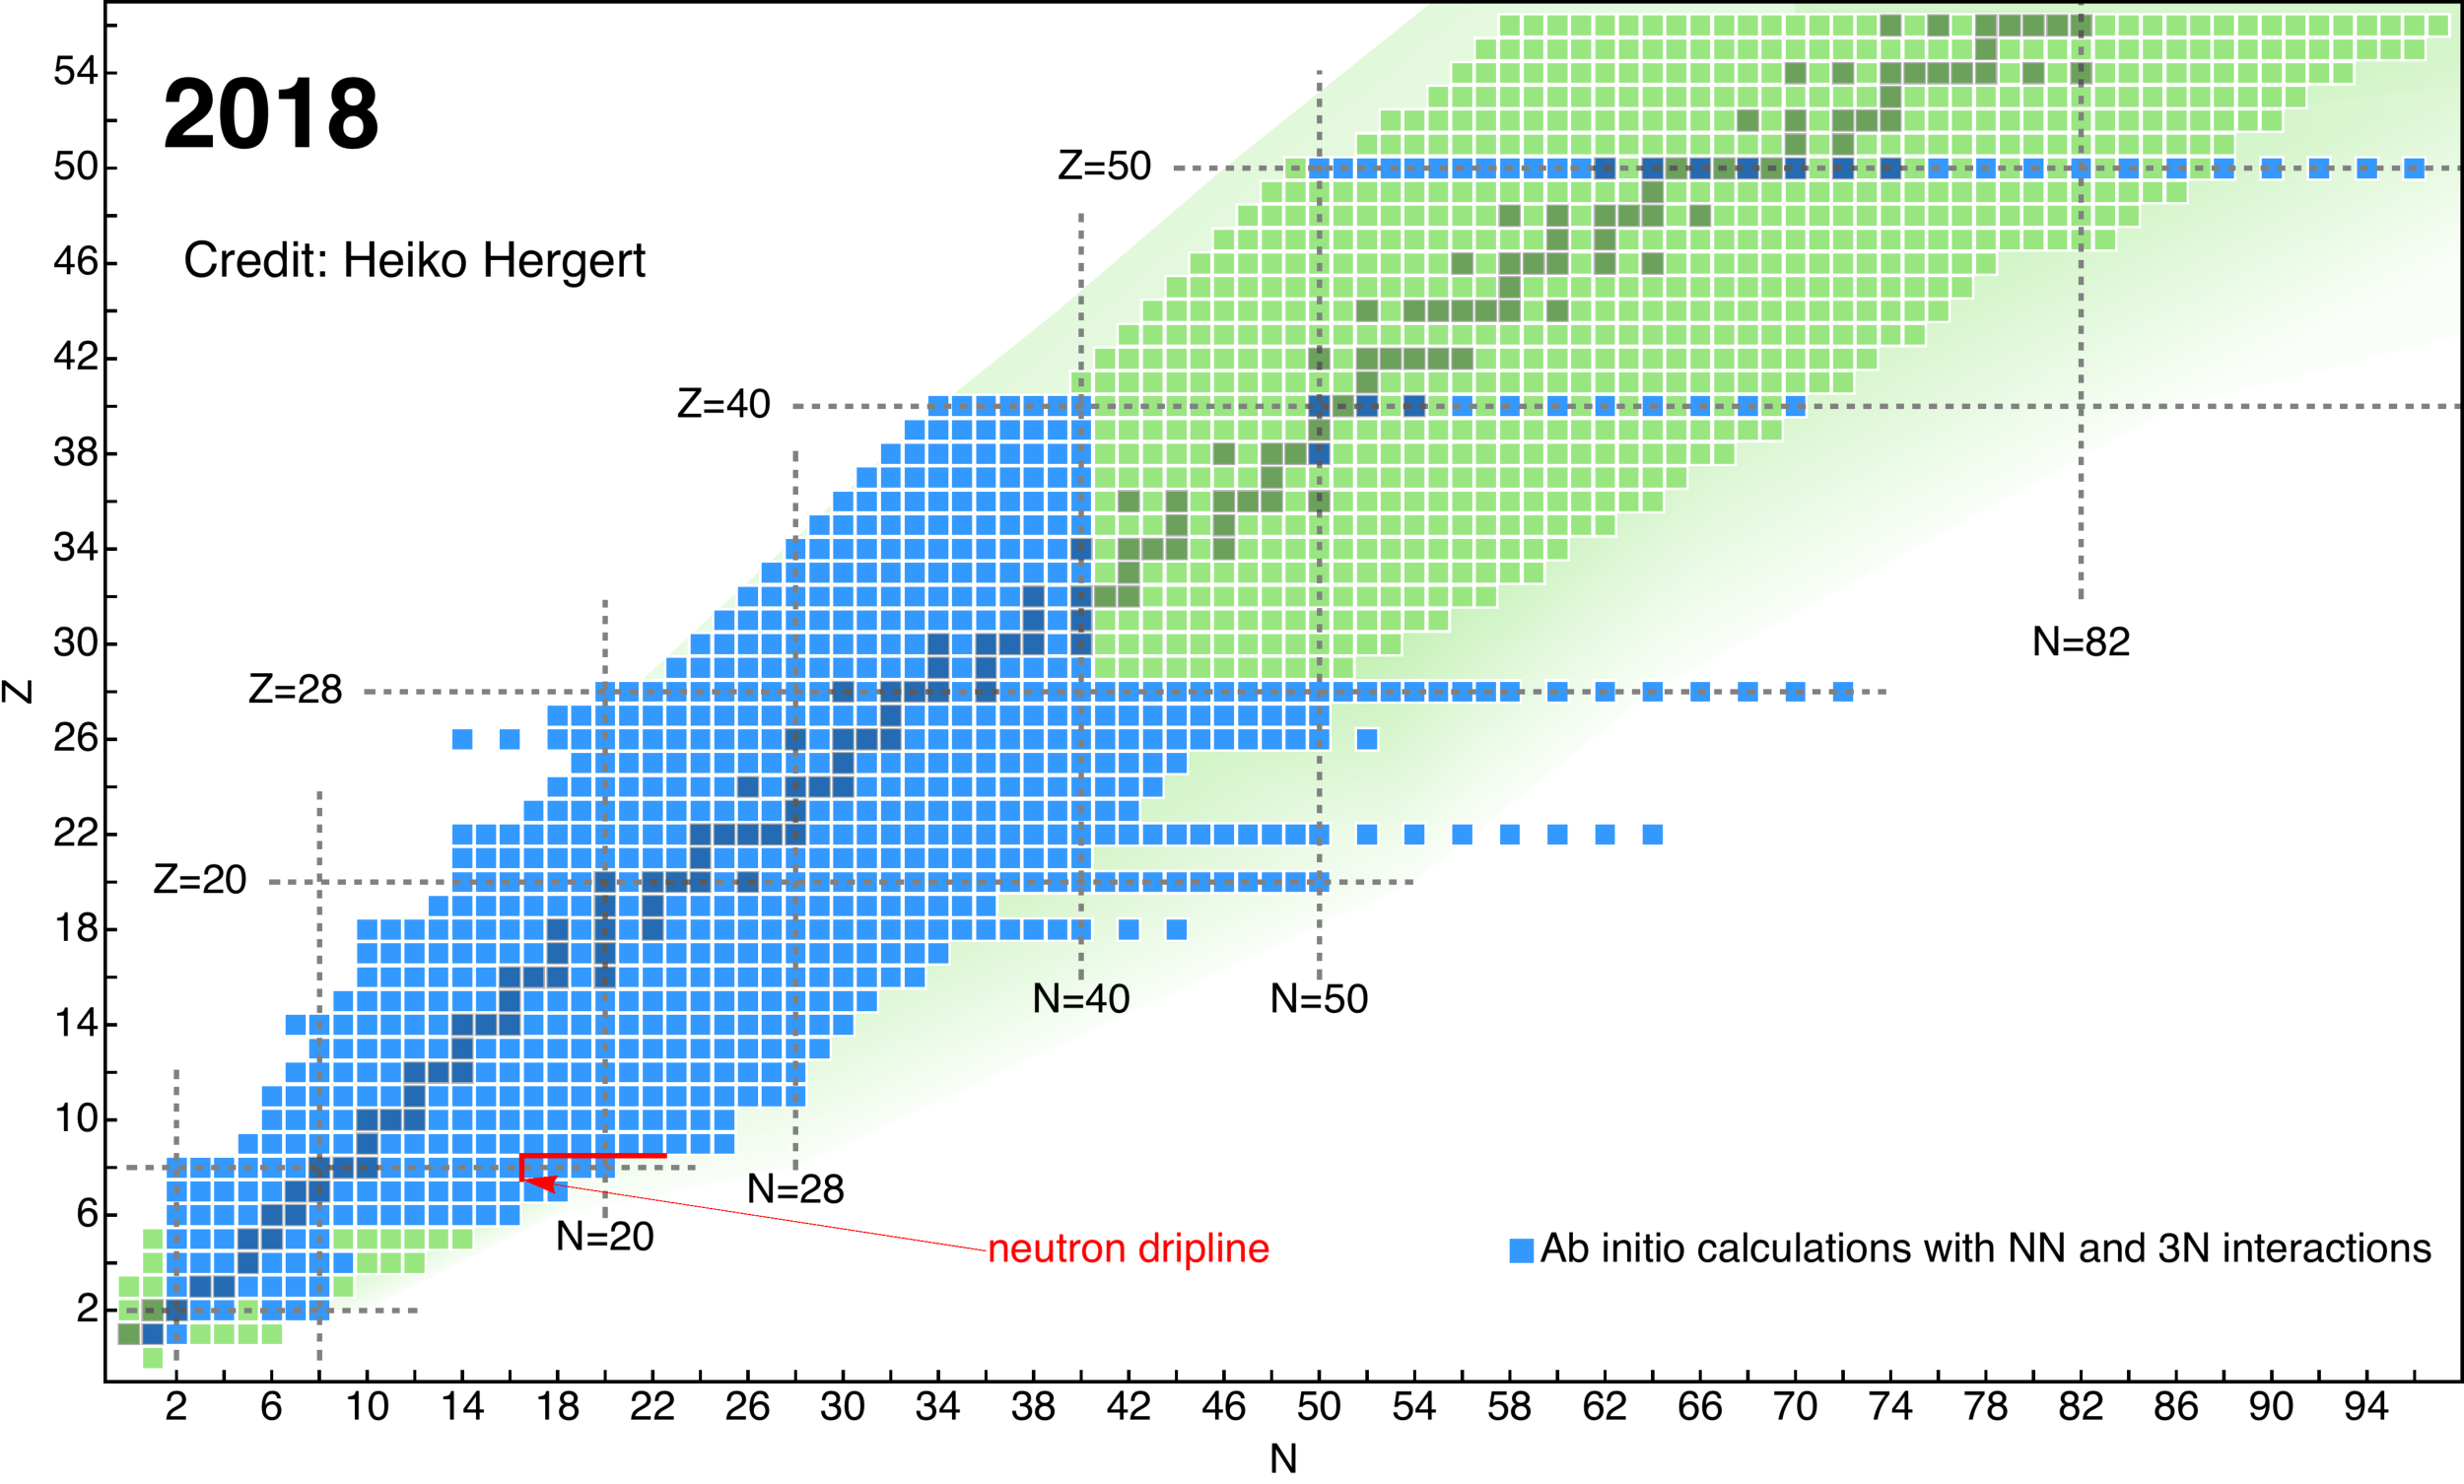
\includegraphics[width=14cm]{nuclear_chart_2018}
	\caption{Chart of nuclides with neutron number, N, counted horizontally and proton number, Z, counted vertically. The green squares correspond to experimentally observed nuclei, whereas the green shaded region depicts the theoretical limits for each isotope. Blue squares correspond to theoretical calculations by \textit{ab initio} methods which will be discussed later. (Figure from H. Hergert.)}
	\label{fig:nuclear_chart_2018}
\end{figure}
%

One such technique is to introduce a complex potential as an effective projectile-nucleus interaction to account for refraction and absorption of the incident particles. These complex potentials are called optical potentials and are used for interpretation of data from reaction experiments. The term optical comes from an analogy where a complex index of refraction is used to describe light refraction and absorption. In nuclear scattering, refraction corresponds to elastic scattering and absorption corresponds to flux disappearing to inelastic channels. Optical potentials have been used to calculate observables of many direct reaction processes and play an important role in the development of nuclear reaction theory \cite{thompson_nunes_2009}.
\\

Originally, optical potentials were constrained by nuclear scattering data to compute effective projectile-nucleus potentials. These phenomenological models are parametrized by fitting scattering observables with parameters such as nuclear radii, diffusivity, etc. Progress in effective field theory (EFT) and renormalization group (RG) methods have led to a wealth of knowledge on the fundamental interaction between nucleons \cite{Epelbaum:2008ga}. We now have access to optical potentials where the interaction between two nucleons (NN force or interaction) is used to compute an effective potential. These potentials are called \textit{ab initio} or microscopic optical potentials. Since microscopic models rely less on scattering data, they offer more predictive power for rare isotopes out of experimental reach.
\\

This paper is organized as follows: in Sec.~\ref{sec:formalism} we present the nuclear optical potential as derived by Feshbach several decades ago \cite{Feshbach:1958nx, Feshbach:1962ut} giving a basic idea of optical potentials conceptually. Sec.~\ref{sec:phenomenology} gives an overview of phenomenological optical potentials and some recent results \cite{Koning:2003zz}. In Sec.~\ref{sec:microscopic} we discuss two \textit{ab initio} approaches to constructing optical potentials and the successes and limitations of these models. Lastly, we summarize and discuss future topics in Sec.~\ref{sec:conclusion}.


%%%%%%%%%%%%%%%%%%%%%%%%%%%%%%%%%%%%%%%%%%%%%%%%%%%%%%%%%%%%%%%%%%%%%%%%%
\section{Formalism}
\label{sec:formalism}


First, we present the optical potential for an $A+1$ particle system consisting of an incident nucleon and a target nucleus of mass number $A$ as derived in \cite{Feshbach:1958nx}. The system is described by the Schr\"odinger equation
%
\begin{eqnarray}
	\label{eq:schrodinger_equation}
	\mathcal{H} \Psi = E \Psi,
\end{eqnarray}
%
with the Hamiltonian $\mathcal{H}$ given below:
%
\begin{eqnarray}
	\label{eq:total_hamiltonian}
	\mathcal{H} = H_A(\textbf{r}_1, \cdots , \textbf{r}_A) + T_0 + V(\textbf{r}_0, \cdots , \textbf{r}_A).
\end{eqnarray}
%
The variables $\textbf{r}_k$ correspond to position, spin, and isospin for the incident nucleon ($k=0$) and each nucleon in the target nucleus ($k=1 \cdots A$). $T_0$ is the kinetic energy of the incident nucleon, and $V$ is the potential energy of the $A+1$ system. $H_A$ is the Hamiltonian for the target nucleus and satisfies the Schr\"odinger equation
%
\begin{eqnarray}
	\label{eq:nuclear_schrodinger_equation}
	H_A(\textbf{r}_1, \cdots , \textbf{r}_A) \psi_i(\textbf{r}_1, \cdots , \textbf{r}_A) = \epsilon_i \psi_i(\textbf{r}_1, \cdots , \textbf{r}_A),
\end{eqnarray}
%
for nuclear wave functions $\psi_i$ and energies $\epsilon_i$. Here, the index $i$ corresponds to each state of the target nucleus with $i=0$ being the ground state. Also, the decomposition of two-, three-, and higher-nucleon interactions in $H_A$ is implicit. The nuclear wave functions $\psi_i$ form a complete, orthonormal set; thus, we can expand the wave function $\Psi$ as follows:
%
\begin{eqnarray}
	\label{eq:wave_function}
	\Psi(\textbf{r}_0, \cdots , \textbf{r}_A) = \sum_{i} \psi_i(\textbf{r}_1, \cdots , \textbf{r}_A) u_i(\textbf{r}_0).
\end{eqnarray}
%
Note, the expansion coefficients $u_i$ carry the $\textbf{r}_0$ dependence. Physically, the expansion coefficients correspond to different outgoing channels with $u_0$ representing elastic scattering.
\\

In the following, we suppress the notation of coordinate, spin, and isospin dependencies for brevity. We substitute Eq.~(\ref{eq:wave_function}) into the Schr\"odinger equation (\ref{eq:schrodinger_equation}) and use the orthonormality of $\psi_i$ to derive a system of equations for the expansion coefficients $u_i$:
%
\begin{eqnarray}
	\label{eq:u_equation}
	(T_0 + V_{ii} + \epsilon_i - E) u_i = - \sum_{j \neq i} V_{ij} u_j,
\end{eqnarray}
%
where the potential matrix elements are
%
\begin{eqnarray}
	\label{eq:potential_matrix_elements}
	V_{ij}(\textbf{r}_0) = \int{d^3 r_1 d^3 r_2 \cdots d^3 r_A \psi_i^* V \psi_j}.
\end{eqnarray}
%
Next, we would like to derive an uncoupled equation for $u_0$ to describe elastic scattering in which the target nucleus is in its ground state with an incident nucleon of energy $E$. The other indices $i$ describe an emergent nucleon in a different state (e.g. energy, spin, isospin, etc.) from the incident nucleon. It is convenient to define the vectors
%
\begin{eqnarray}
	\label{eq:u_vector}
	\Phi \equiv
	\begin{pmatrix}
		u_1 \\
		u_2 \\
		\vdots \\
	\end{pmatrix}
	,
\end{eqnarray}
%
\begin{eqnarray}
	\label{eq:potential_vector}
	\textbf{V}_0 =
	\begin{pmatrix}
		V_{01}, V_{02}, \cdots
	\end{pmatrix}
	,
\end{eqnarray}
%
and the matrix operator $\textbf{H}$
%
\begin{eqnarray}
	\label{eq:hamiltonian_operator}
	H_{ij} = T_0 \delta_{ij} + V_{ij} + \epsilon_i \delta_{ij},
\end{eqnarray}
%
for $i$, $j > 0$. Then we can rewrite (\ref{eq:u_equation}) as
%
\begin{subequations}
	\label{eq:u_vector_equation}
	\begin{eqnarray}
		\label{eq:u_vector_equation_a}
		(T_0 + V_{00} - E) u_0 = -\textbf{V}_0 \Phi,
	\end{eqnarray}
	\begin{eqnarray}
		\label{eq:u_vector_equation_b}
		(\textbf{H}-E) \Phi = -\textbf{V}_0^{\dagger} u_0.
	\end{eqnarray}
\end{subequations}
%
We solve (\ref{eq:u_vector_equation_b}) for $\Phi$
%
\begin{eqnarray}
	\label{eq:phi}
	\Phi = \frac{1}{E - \textbf{H} + i \eta} \textbf{V}_0^{\dagger} u_0,
\end{eqnarray}
%
where $\eta \rightarrow 0^+$ to ensure only outgoing waves are present in exit channels for $u_i$ with $i \geq 1$. Lastly, we substitute $\Phi$ into (\ref{eq:u_vector_equation_a}) to give
%
\begin{eqnarray}
	\label{eq:u0_equation}
	(T_0 + V_{00}  - \textbf{V}_0 \frac{1}{E-\textbf{H}+i\eta} \textbf{V}_0^{\dagger} - E) u_0 = 0,
\end{eqnarray}
%
and define the optical potential as
%
\begin{eqnarray}
	\label{eq:optical_potential}
	V_{opt} = V_{00}  + \textbf{V}_0 \frac{1}{E-\textbf{H}+i\eta} \textbf{V}_0^{\dagger}.
\end{eqnarray}
%
\\

We can see from Eq.~(\ref{eq:optical_potential}) that the optical potential is complex and energy dependent. The factor of $i \eta$ leads to $V_{opt}$ being complex, and thus, non-hermitian. It also accounts for incident particles leaving the entrance channel $u_0$ to an exit channel $u_i$ where $i \geq 1$. This only occurs if reactions are possible, that is, $E > \epsilon_1$. Because $V_{opt}$ is non-hermitian, the $S$-matrix is not unitary giving rise to complex scattering phase shifts. Furthermore, the potential is non-local from the second term. We can see the non-locality by acting the operator $V_{opt}$ on a wave function $\Psi$ in coordinate-space, giving an integral over the surrounding region. Mathematically, this corresponds to a term $\int d^3 r' \, V(\textbf{r}, \textbf{r}') \Psi(\textbf{r}')$ in the Schr\"odinger equation \cite{Hodgson:1971ab}. The derivation only accounts for one nucleon in the exit channel, and thus, does not describe all types of reactions. Feshbach generalized the approach by using projection operators in \cite{Feshbach:1962ut} which is summarized below.
\\

Here, we define the two projection operators $P$ and $Q$. $P$ projects the total wave function onto the ground state of the target wave function: $P \Psi = \psi_0 u_0$. $Q$ projects onto all other states and is given by $Q = 1-P$. The projection operators satisfy the following relations: $P+Q=1$, $P^2 = P$, $Q^2 = Q$, and $P Q = 0$. We act on Eq.~(\ref{eq:schrodinger_equation}) with $P$ and $Q$, and use the projection operator relations to obtain two equations:
%
\begin{subequations}
	\label{eq:intermediate_effective_hamiltonian_equations}
	\begin{eqnarray}
		\label{eq:pp_pq}
		(E - \mathcal{H}_{PP}) P \Psi = \mathcal{H}_{PQ} Q \Psi,
	\end{eqnarray}
	\begin{eqnarray}
		\label{eq:qq_qp}
		(E - \mathcal{H}_{QQ}) Q \Psi = \mathcal{H}_{QP} P \Psi,
	\end{eqnarray}
\end{subequations}
%
where $\mathcal{H}_{PP}$ refers to $P \mathcal{H} P$ and so forth. Solving (\ref{eq:qq_qp}) for $Q \Psi$ yields
%
\begin{eqnarray}
	\label{eq:q_psi}
	Q \Psi = \frac{1}{E - \mathcal{H}_{QQ} + i \eta} \mathcal{H}_{QP} P \Psi.
\end{eqnarray}
%
Substituting $Q \Psi$ into Eq.~(\ref{eq:pp_pq}) and rearranging gives
%
\begin{eqnarray}
	\label{eq:p_psi}
	(E - \mathcal{H}_{PP} - \mathcal{H}_{PQ} \frac{1}{E - \mathcal{H}_{QQ} + i \eta} \mathcal{H}_{QP}) P \Psi = 0.
\end{eqnarray}
%
By taking the ground state of the target nucleus to be zero, $H_A \psi_0 = 0$,  and using $P = \ket{\psi_0} \bra{\psi_0}$, one can show that Eq.~(\ref{eq:p_psi}) becomes
%
\begin{eqnarray}
	\label{eq:p_psi_optical_potential}
	(E - T - \mel{\psi_0}{V}{\psi_0} - \mel{\psi_0}{V Q \frac{1}{E - \mathcal{H}_{QQ} + i \eta} Q V}{\psi_0}) u_0 = 0,
\end{eqnarray}
%
similar to Eq.~(\ref{eq:u0_equation}). We identify the optical potential as
%
\begin{eqnarray}
	\label{eq:optical_potential_projection}
	V_{opt} = \mel{\psi_0}{V}{\psi_0} + \mel{\psi_0}{V Q \frac{1}{E - \mathcal{H}_{QQ} + i \eta} Q V}{\psi_0},
\end{eqnarray}
% 
where the first term corresponds to pure elastic scattering, and the second term corresponds to virtual nuclear excitations and de-excitations back to the elastic channel. Note, this is technically the same as Eq.~(\ref{eq:optical_potential}), as the inner products are written out explicitly in Eq.~(\ref{eq:optical_potential_projection}) and denoted with subscripts in Eq.~(\ref{eq:optical_potential}). Also, the two vector terms $\textbf{V}_0$ in the original equation account for couplings of the elastic channel to inelastic channels, while this is done with the $Q$ projection operator in the second definition of the optical potential.


%%%%%%%%%%%%%%%%%%%%%%%%%%%%%%%%%%%%%%%%%%%%%%%%%%%%%%%%%%%%%%%%%%%%%%%%%
\section{Phenomenology}
\label{sec:phenomenology}


Historically, phenomenological optical potentials have been obtained by fitting elastic-scattering angular distributions with a complex potential of the form \cite{Perey:1976zz, Dickhoff:2018wdd}
%
\begin{eqnarray}
	\label{eq:phenomenological_optical_potential}
	V_{opt}(r, E) &=& V_C(r) - V(E) f(x_0) + (\frac{\hbar}{m_{\pi} c})^2 V_{SO}(E) \bm{\sigma} \cdot \textbf{l} \frac{1}{r} \frac{d}{dr} f(x_{SO}) \nonumber \\ 
& &- i [W(E) f(x_W) - 4 W_D(E) \frac{d}{dx_D} f(x_D)].
\end{eqnarray}
%
Here, $f(x_i) = (1 + \exp[x_i])^{-1}$ are Woods-Saxon form factors dependent on the radii and diffusivity parameters, $R_i$ and $a_i$, where $x_i = \frac{r-R_i}{a_i}$. The index $i$ specifies each of the terms above (e.g. $C$, $0$, $SO$, etc.), $a_i$ is the diffusivity, and $R_i = r_i A^{1/3}$ is the nuclear radius. Nuclear radii are roughly proportional to $A^{1/3}$, hence the form of $R_i$. Woods-Saxon potentials have been used to describe the mean field potential of a nucleon in a nucleus, thus serve as good candidates for modeling the projectile-nucleus interaction. (A mean field potential is a potential that averages over the interactions of a system reducing a many-body problem to a one-body problem.)
\\

The first term, $V_C$, accounts for charged-interactions between charged particles (e.g. an incident proton and a nuclear target with total charge $Z'$) where
%
\begin{eqnarray}
	\label{eq:coulomb_potential}
	V_C =
	\begin{cases}
		\frac{Z Z' e^2}{r} \qquad \text{if $r \geq R_C$} \\
		\frac{Z Z' e^2}{2 R_C} (3 - \frac{r^2}{R_C^2}) \qquad \text{if $r \leq R_C$}.
	\end{cases}
\end{eqnarray}
%
This is the Coulomb potential of a spherical, uniformly-charged distribution of radius $R_C$. Note, this term is zero if the projectile particles are neutral (e.g. incident neutrons). The $V$ term gives the approximate interaction between the incident particle and the target nucleus and typically has a potential well depth of $V \approx 50$ MeV. $V_{SO}$ is the spin-orbit coupling term where $\bm{\sigma}$ is the spin operator and $\bm{l}$ is the angular momentum of the incident particle and is important for describing analyzing powers (scattering observables related to spin-dependent cross sections).
\\

At higher energies, an imaginary component is necessary to describe absorption where particles penetrate into and through the target nucleus. The first term, $W$, represents volume absorption, and the second, $W_D$, surface absorption. These components include a Woods-Saxon form factor and its derivative, respectively. Note, the derivative of the Woods-Saxon function peaks at the nuclear radius, hence the $W_D$ accounting for surface absorption. At lower energies ($E < 10$ MeV) the surface term dominates while at higher energies one must include the volume absorption component. In Fig.~\ref{fig:potential_wells_omp}, we show examples of the energy dependent terms in Eq.~(\ref{eq:phenomenological_optical_potential}).
\\

%
\begin{figure}
	\captionsetup{singlelinecheck=false,justification=raggedright}
	\centering
	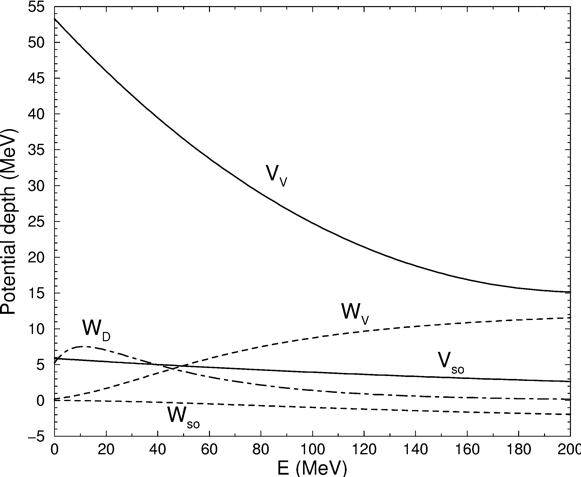
\includegraphics[width=10cm]{potential_wells_omp}
	\caption{Potential well depths as a function of laboratory energy $E$ for each of the terms in Eq.~\ref{eq:phenomenological_optical_potential} including an imaginary spin-orbit term, $W_{SO}$ \cite{Koning:2003zz}.}
	\label{fig:potential_wells_omp}
\end{figure}
%

Phenomenological optical potentials are often obtained by $\chi^2$ minimization fitting angular distributions, analyzing powers, or cross section with radii and diffusivity parameters. The $\chi^2$ function is dependent on experimental data which can heavily affect the fitted parameters depending on which data sets are used or the methodology to arrive at an average data set. In many situations, several sets of parameters can give a good fit to experimental data. Furthermore, optical models may have differing definitions of the $\chi^2$ function. Overall, this leads to an ambiguity in fitting an optical potential model. In the remainder of this section, we discuss three methods in parameterizing a phenomenological optical potential: best-fit, global-fit, and local-fit.
\\

A best-fit optical model is a model fit from one set of data (e.g. a single elastic angular distribution). With several parameters to obtain a satisfactory fit, these models can adequately describe a specific projectile and nuclear target. However, parameter sets from best-fit models are energy dependent and fail to make predictions at energies outside the range of data. The only recent use of best-fit models are to provide insight in global trends for optical model parameters across different energy ranges, and thus serve as a preliminary step for parameterizing either local or global optical models.
\\

A global-fit model is the opposite of the best-fit model in the sense that global-fit models cover wide ranges of energy and mass number $A$. In this way, we can expect better predictive power from these models for nuclei where no experimental data exist. These parameterizations require a large range of data sets to give an ``average'' description of the projectile-nucleus interaction. However, these models are often unreliable since different nuclei are not smoothly dependent on $A$ or $Z$, unlike the Woods-Saxon parameters. This fault advocates the development of microscopic optical potentials which can consistently describe the interaction for various nuclei.
\\

Lastly, the local-fit models are a combination of the former methods. Here, parameters are specific to a given target nucleus with energy-dependence expressed analytically. The parameters are fit by varying them around global-fit parameters for each nucleus of interest. The resulting parameters are similar for neighboring nuclei; however, the variation in parameters is still unpredictable. An example of a recent local-fit optical potential is given in \cite{Koning:2003zz}.
\\

Phenomenological models have been successful in describing scattering from nuclei where data are available; however, the approach lacks realistic nuclear structure inputs like multi-pion exchange contributions, three-body interactions, etc. Without including these details, phenomenological models cannot make consistent predictions across all scattering systems or extend to exotic nuclei. Furthermore, there is no reliable way to quantify uncertainty in these models. In the next section, we discuss microscopic optical potentials which seek to overcome the shortcomings of the phenomenological models.


%%%%%%%%%%%%%%%%%%%%%%%%%%%%%%%%%%%%%%%%%%%%%%%%%%%%%%%%%%%%%%%%%%%%%%%%%
\section{Microscopic optical potentials}
\label{sec:microscopic}


In this section, we present two methods to calculate microscopic optical potentials: the multiple-scattering approach and nucleon self-energy methods. As previously mentioned, it is important to have a theoretical grasp on applying microscopic NN potentials to the optical potential methodology in order to make predictions where no experimental data are available. Groups have attempted to fit global optical potentials to accomplish this goal but fail to consistently match experimental observables across several nuclei and energies primarily because of the lack of nuclear structure inputs to their models. Recently, a number of methods have been developed to calculate microscopic optical potentials \cite{Furumoto:2019anr, Idini:2019hkq, Rotureau:2016jpf}.


%___________________________________________________________________________________________________________________
\subsection{Multiple-scattering approach}
\label{sec:multiple_scattering}


The multiple-scattering approach includes important multiple-scattering events in the NN $T$-matrix which is used to calculate the optical potential. The NN $T$-matrix uses pairwise interactions between the projectile particle and nucleons with realistic NN forces derived from \textit{ab initio} methods. We derive the optical potential using this approach following the notation in \cite{Dickhoff:2018wdd} and \cite{Burrows:2018ggt}.
\\

First, we assume two-particle interactions between the projectile and a single nucleon within the target nucleus dominate. Then we can write the interaction between the projectile and the nucleus as a sum of all pairwise interactions:
%
\begin{eqnarray}
	\label{eq:ms_total_potential}
	V = \sum_{i=1}^A V(0, i),
\end{eqnarray}
%
where the arguments in the parentheses indicate the interaction between the projectile ($0$) and a nucleon ($i$). (Note, one can include three-nucleon forces (3NF's) at this step.) Then the Hamiltonian of the $A+1$ system can be written with the approximated potential (\ref{eq:ms_total_potential})
%
\begin{eqnarray}
	\label{eq:ms_hamiltonian}
	\mathcal{H} = H_0 + H_A + \sum_{i=1}^A V(0, i) = \mathcal{H}_0 + \sum_{i=1}^A V(0, i),
\end{eqnarray}
%
where $\mathcal{H}_0$ gives the energy of the non-interacting projectile and nucleus. The $T$-matrix for elastic scattering from the nuclear target's ground state is
%
\begin{eqnarray}
	\label{eq:tmatrix}
	T = V + V G_0(E) T,
\end{eqnarray}
%
where the Green's function is given by $G_0(E) = \frac{1}{E - \mathcal{H}_0 + i \eta}$.
\\

For elastic scattering, we re-introduce the projection operators from before, $P$ and $Q$, and re-write (\ref{eq:tmatrix})
%
\begin{eqnarray}
	\label{eq:tmatrix_elastic}
	T = U + U G_0(E) P T,
\end{eqnarray}
%
where the optical potential $U$ describes elastic scattering:
%
\begin{eqnarray}
	\label{eq:ms_optical_potential_elastic}
	U = V + V G_0(E) Q T,
\end{eqnarray}
%
and the full elastic-scattering $T$-matrix is
%
\begin{eqnarray}
	\label{eq:tmatrix_full_elastic}
	T_{el} = P U P + P U P G_0(E) P T_{el}.
\end{eqnarray}
%
Now we apply the so-called spectator expansion to the optical potential $U$:
%
\begin{eqnarray}
	\label{eq:spec_exp}
	U = \sum_{i=1}^A \tau(0, i) + \sum_{i \neq j}^A \tau(0, i) Q G_0(E) \tau(0, j) + \cdots,
\end{eqnarray}
%
where
\begin{eqnarray}
	\label{eq:tau_equations}
	\tau(0, i) &=& V(0, i) + V(0, i) G_0(E) Q \tau(0, i) = \hat{\tau}(0, i) - \hat{\tau}(0, i) G_0(E) P \tau(0, i),
\end{eqnarray}
%
with the reduced amplitudes $\hat{\tau}(0, i) = V(0, i) + V(0, i) G_0(E) \hat{\tau}(0, i)$. The spectator expansion orders the scattering processes in a sequence of projectile-target interactions. The first term corresponds to the projectile interacting with one nucleon while the rest are spectators depicted in Fig.~\ref{fig:single_scattering}. The second term corresponds to the projectile interacting with two nucleons and so forth. We make the simplest approximation and take only the first term in the expansion called the impulse approximation. The impulse approximation is valid when the energy of the incident particle is much larger than the binding potential of the struck nucleon ($E > 100$ MeV). Also, 3NF's do not contribute in the impulse approximation since it only takes projectile-nucleon interactions into account.
\\

%
\begin{figure}
	\captionsetup{singlelinecheck=false,justification=raggedright}
	\centering
	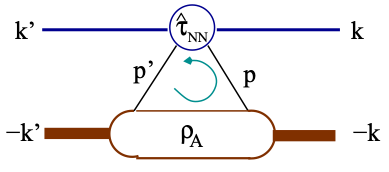
\includegraphics[width=8cm]{single_scattering}
	\caption{Diagram of the single scattering term in the spectator expansion where the momentum variables are defined below \cite{Burrows:2018ggt}.}
	\label{fig:single_scattering}
\end{figure}
%

Next, we introduce the momentum variables
%
\begin{subequations}
	\label{eq:momenta}
	\begin{eqnarray}
		\label{eq:momentum_transfer}
		\textbf{q} = \textbf{k}' - \textbf{k},
	\end{eqnarray}
	\begin{eqnarray}
		\label{eq:total_momentum}
		\textbf{K} = \frac{1}{2} ( \textbf{k} + \textbf{k}' ),
	\end{eqnarray}
	\begin{eqnarray}
		\label{eq:internal_momentum}
		\textbf{P} = \frac{1}{2} ( \textbf{p} + \textbf{p}' ),
	\end{eqnarray}
\end{subequations}
%
which correspond to momentum transfer, total momentum, and total internal momentum of nucleons, given initial and final momenta $\textbf{k}$ and $\textbf{k}'$, respectively (see Fig.~\ref{fig:single_scattering}). We can write the optical potential in momentum-space as a convolution of the effective interaction with the target's ground state:
%
\begin{eqnarray}
	\label{eq:ms_optical_potential}
	U(\textbf{q}, \textbf{K}; E) = \sum_{\alpha = p, n} \int d^3 P \, \eta(\textbf{P}, \textbf{q}, \textbf{K}) \hat{\tau}_{\alpha}(\textbf{k}, \textbf{k}') \rho_{\alpha}(\textbf{P} - (A-1) \frac{\textbf{q}}{2 A}, \textbf{P} + (A-1) \frac{\textbf{q}}{2 A}),
\end{eqnarray}
%
where $\eta$, the M\o ller factor, relates the NN zero-momentum frame to the NA zero-momentum frame (details in \cite{Elster:1996xh}), and $\rho_{\alpha}$ represents the one-body density matrix (proton and neutron densities). There are several ways to calculate the $T$-matrix and one-body density matrix $\rho$. Recent studies have used the No-Core Shell Model (NCSM) method to calculate the density matrix which allows for a consistent NN interaction between the density matrix and $T$-matrix (\cite{Burrows:2018ggt, Gennari:2017yez}). It is possible to further simplify Eq.~(\ref{eq:ms_optical_potential}) by making the $\tau \rho$ approximation, which involves writing the potential where the density $\rho$ does not depend on the total internal momentum $\textbf{P}$, and the NN $T$-matrix and the M\o ller factor determine the non-local character of the potential.
\\

%
\begin{figure}
	\captionsetup{singlelinecheck=false,justification=raggedright}
	\centering
	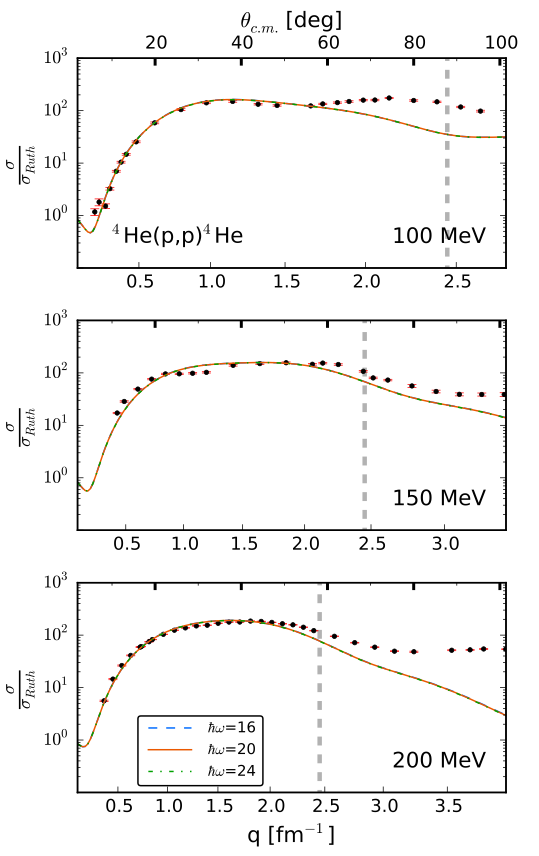
\includegraphics[width=8cm]{burrows_figure}
	\caption{Differential cross section divided by Rutherford cross section for elastic scattering of protons from $^{4}$He at lab energies $100$ (top), $150$ (middle), and $200$ (bottom) MeV. The lower axes show the momentum transfer $q$ and the upper axes show the center-of-mass angle. Lastly, the values of $\hbar \omega$ serve as inputs to the NCSM, and dashed vertical lines indicate the momentum transfer $q = 2.45$ fm$^{-1}$ corresponding to the lab energy $125$ MeV of the $np$ system \cite{Burrows:2018ggt}.}
	\label{fig:burrows_figure}
\end{figure}
%

Fig.~\ref{fig:burrows_figure} shows cross section results for elastic proton scattering from $^{4}$He using the multiple-scattering approach. Overall, the multiple-scattering approach at first order describes experiments well in the energy range of $100$ to $200$ MeV and up to roughly $60$ degrees in the center-of-mass frame. At angles larger than this, 3NF's become important due to three-body scattering. Unfortunately, the implementation of 3NF's is challenging as including an extra term in Eq.~(\ref{eq:ms_total_potential}) forces one to take another term in the spectator expansion (\ref{eq:spec_exp}).
		
	
%___________________________________________________________________________________________________________________
\subsection{Nucleon self-energy with chiral interactions}
\label{sec:nucleon_self_energy}

There has been recent interest in the development of microscopic optical potentials based on chiral effective field theory, $\chi^{EFT}$. We will present the nucleon self-energy method from this perspective. In quantum many-body physics, the optical potential for scattering states is identified with the energy- and momentum-dependent single particle self-energy. Particle self-energy is the modification to particle energy due to interactions with its environment (in this case, the nuclear medium) and is used in many-body perturbation theory. We will denote self-energy with $\Sigma$. Here, the basic idea is to calculate the nucleon self-energy in nuclear matter using chiral interactions. First, we give a brief description of $\chi^{EFT}$.
\\

In $\chi^{EFT}$, chiral perturbation theory is applied to nuclear systems and gives an EFT involving nucleons and Goldstone bosons, which are pions, due to chiral symmetry breaking. This gives a low-energy description of the nuclear force with proton, neutron, and pion degrees of freedom with protons and neutrons interacting by pion exchanges and contact forces. The theory contains long- and short-range terms where the long-range terms (pion exchanges) are calculated explicitly, and the short-range terms (contact forces) are parameterized by NN scattering data. Chiral interactions can be softened by RG transformations to overcome obstacles in many-body calculations often due to the hard repulsive core in the NN force. However, being an effective field theory, a regularization procedure is necessary to separate high- and low-energy physics. At high energies, the theory is no longer valid and a cutoff must be introduced. From the optical potential perspective, this offers a trade-off. These theories are well suited to describe low-energy scattering but fail at energies near or above the momentum-space cutoff employed.
\\

%
\begin{figure}
	\captionsetup{singlelinecheck=false,justification=raggedright}
	\centering
	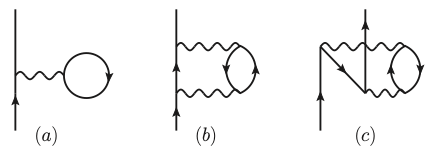
\includegraphics[width=10cm]{nucleon_self_energy}
	\caption{First- and second-order contributions to the nucleon self-energy where the solid lines indicate nucleon propagators and the wavy lines indicate the in-medium, anti-symmetrized NN interaction \cite{Whitehead:2018bfs}.}
	\label{fig:nucleon_self_energy}
\end{figure}
%

We derive an optical potential by computing the nucleon self-energy in nuclear matter using chiral interactions following the formalism of \cite{Whitehead:2018bfs, Holt:2013tna}. The first two perturbative contributions to the nucleon self-energy are shown in Fig.~\ref{fig:nucleon_self_energy} and are given by
%
\begin{eqnarray}
	\label{eq:nucleon_self_energy_1}
	\Sigma_{2N}^{(1)} (q; k_f) = \sum_i \mel{\textbf{q} \textbf{h}_i s s_i t t_i}{V_{2N}^{eff}}{\textbf{q} \textbf{h}_i s s_i t t_i} n_i,
\end{eqnarray}
%
\begin{eqnarray}
	\label{eq:nucleon_self_energy_2a}
	\Sigma_{2N}^{(2a)} (q, \omega; k_f) = \frac{1}{2} \sum_{ijk} \frac{|\mel{\textbf{p}_i \textbf{p}_k s_i s_k t_i t_k}{V_{2N}^{eff}}{\textbf{q} \textbf{h}_j s s_j t t_j}|^2}{\omega+\epsilon_j-\epsilon_i-\epsilon_k+i \eta} \bar{n}_i n_j \bar{n}_k,
\end{eqnarray}
%
\begin{eqnarray}
	\label{eq:nucleon_self_energy_2b}
	\Sigma_{2N}^{(2b)} (q, \omega; k_f) = \frac{1}{2} \sum_{ijk} \frac{|\mel{\textbf{h}_i \textbf{h}_k s_i s_k t_i t_k}{V_{2N}^{eff}}{\textbf{q} \textbf{p}_j s s_j t t_j}|^2}{\omega+\epsilon_j-\epsilon_i-\epsilon_k-i \eta} n_i \bar{n}_j n_k,
\end{eqnarray}
%
where $n_i$ is the occupation probability $\theta(k_f - k_i)$ for a filled state with momentum $\textbf{k}_i$ below the Fermi-surface, and the occupation probability for particle states is $\bar{n}_i = 1 - n_i$. The summations are over intermediate-state momenta for particles $\textbf{p}_i$ and holes $\textbf{h}_i$, their spins $s_i$, and isospins $t_i$ The energies are calculated self-consistently with $\epsilon_i = \frac{q^2}{2 M} + \Re \Sigma(q, \epsilon(q))$ where $M$ is the mass of the nucleon.
\\

The effective potentials $V_{2N}^{eff}$ consist of an NN potential with an effective, medium-dependent NN interaction. The medium-dependent interaction depends on the chiral three-nucleon force. The Hartree-Fock contribution (\ref{eq:nucleon_self_energy_1}) is non-local, energy-independent, and real, whereas the next two terms (\ref{eq:nucleon_self_energy_2a} and \ref{eq:nucleon_self_energy_2b}) are non-local, energy dependent, and complex. The optical potential is  then given by
%
\begin{eqnarray}
	\label{eq:nucleon_self_energy_optical_potential}
	U_N(E; k_f^p, k_f^n) = V_N(E; k_f^p, k_f^n) + i W_N(E; k_f^p, k_f^n),
\end{eqnarray}
%
where
\begin{eqnarray}
	\label{eq:nucleon_self_energy_optical_potential_real}
	V_N(E; k_f^p, k_f^n) = \Re \Sigma_i (q, E(q); k_f^p, k_f^n),
\end{eqnarray}
%
\begin{eqnarray}
	\label{eq:nucleon_self_energy_optical_potential_imaginary}
	W_N(E; k_f^p, k_f^n) = \frac{M_N^{k*}}{M} \Im \Sigma_i (q, E(q); k_f^p, k_f^n),
\end{eqnarray}
%
where the subscript, $N$, refers to a propagating proton or nucleon. Here, $M_N^{k*}$ is the nucleon effective $k$-mass defined by $\frac{M_N^{k*}}{M} = (1+\frac{M}{k} \frac{\partial}{\partial k} V_N(k, E(k)))^{-1}$.
\\

%
\begin{figure}
	\captionsetup{singlelinecheck=false,justification=raggedright}
	\centering
	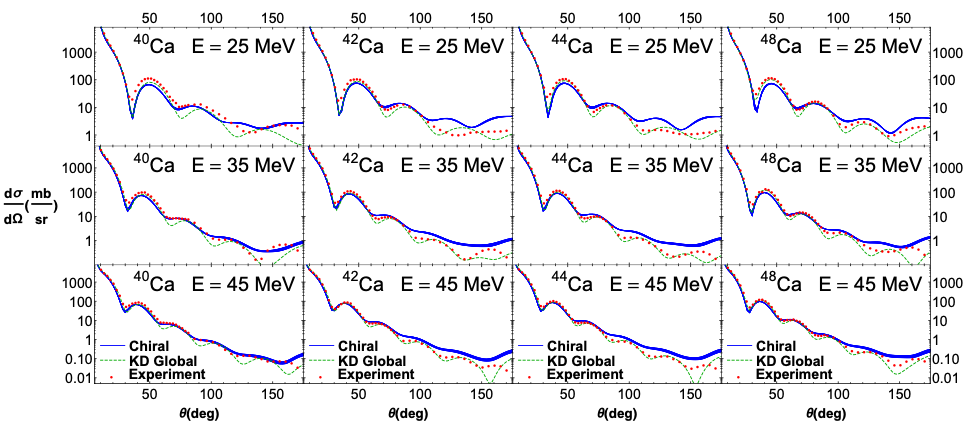
\includegraphics[width=15cm]{whitehead_figure}
	\caption{Differential cross section for elastic scattering of protons from calcium isotopes at lab energies $25$ (top), $35$ (middle), and $45$ (bottom) MeV. Blue lines correspond to the microscopic cross sections, green lines to a global phenomenological model, and red circles to experimental data \cite{Whitehead:2018bfs}.}
	\label{fig:whitehead_figure}
\end{figure}
%

Fig. \ref{fig:whitehead_figure} shows cross section results using this method. We see good agreement between the chiral approach and data at forward scattering angles and slight deviation at larger angles. Optical models built from chiral interactions are well-suited to describe low-energy scattering data. As mentioned before, the momentum-space cutoff of the effective field theory limits the capability of these models. Therefore, we expect chiral models to break down for energies approaching the cutoff employed. Typically, this limits these models to $E < 200$ MeV.


%%%%%%%%%%%%%%%%%%%%%%%%%%%%%%%%%%%%%%%%%%%%%%%%%%%%%%%%%%%%%%%%%%%%%%%%%
\section{Conclusion}
\label{sec:conclusion}


In summary, we described nuclear optical potentials as originally presented by Feshbach several decades ago. We discussed the history and current use of phenomenological models focusing on the advantages and disadvantages of different approaches. Overall, phenomenological models are restricted to describing systems where sufficient experimental data are present. This shortcoming warrants the development of theoretical approaches built from our current understanding of the nuclear force. We briefly presented two such approaches in Sec.~\ref{sec:microscopic}: the multiple-scattering approach and the nucleon self-energy approach. The former adequately describes scattering data up to high energies and large scattering angles. The implementation of 3NF's in multiple-scattering approaches is difficult and limits these models. However, in some cases, it is possible to consistently calculate the $T$-matrix and nuclear density which is a major advantage. The nucleon self-energy approach presented is largely limited by the underlying chiral interactions. Using chiral interactions allows for implementation of realistic interactions like pion exchanges, three-body interactions, and a means to quantify theoretical uncertainty estimates. Lastly, there are many microscopic approaches not covered in this paper such as the nuclear matter approach by Jeukenne, Lejeune, and Mahaux \cite{Jeukenne:1977zz} or Green's function based methods \cite{Dickhoff:2018wdd}. The reader may refer to these references for details.
\\

Despite the progress, microscopic models still face some of the challenges that global phenomenological models face in that they can be too imprecise across kinematic ranges or nuclei. However, current microscopic models can be used to guide phenomenological models, for instance, on the functional form of potential well depths. It is necessary to further understand what components are key in computing an \textit{ab initio} optical potential such as the effect of higher-body interactions or being able to reproduce nuclear structure observables like radii. Work is also being done on understanding uncertainty quantification for optical potential models \cite{King:2018vzw}. With a stronger grasp on uncertainty quantification, different models can be reliably compared. Another area of interest involves an RG method called the Similarity Renormalization Group (SRG) which started as a way to soften NN potentials while preserving the underlying observables \cite{Bogner:2006pc, Bogner:2009bt}. Scattering observables are process-independent quantities but inherit scheme dependence from the factorization of nuclear structure from the scattering probe. Recently, the SRG was used to analyze a simple knockout reaction, deuteron electrodisintegration, to gain insight on the scheme dependence. It would be interesting to apply the same idea to optical potential models to investigate scheme dependence and the validity of common approximations.


%%%%%%%%%%%%%%%%%%%%%%%%%%%%%%%%%%%%%%%%%%%%%%%%%%%%%%%%%%%%%%%%%%%%%%%%%


\bibliography{../../tropiano_bib}


\end{document}